\section{Multigraphs and Digraphs}
There are occasions when graphs may not be an appropriate model for a problem we are investigating. We now describe two variations of graphs that we will encounter from time to time. In a graph, two vertices are either adjacent or they are not, that is, two vertices are joined by one edge or no edges. A \bf{multigraph} $M$ consists of a finite nonempty set $V$ of vertices and a set $E$ of edges, where every two vertices of $M$ are joined by a finite number of edges (possibly zero). If two or more edges join the same pair of (distinct) vertices, then these edges are called \bf{parallel edges}. In a \bf{pseudograph}, not only are parallel edges permitted but an edge is also permitted to join a vertex to itself. Such an edge is called a \bf{loop}. If a loop $e$ joins a vertex $v$ to itself, then $e$ is said to be a loop at $v$. There can be any finite number of loops at the same vertex in a pseudograph. In Figure 1.35, $M_{1}$ and $M_{2}$ are multigraphs, $M_{3}$ is a pseudograph and $M_{4}$ is a graph. In fact, $M_{4}$ is a multigraph and all four are pseudographs.

\begin{figure}[h]
	\centering
	\captionsetup[subfigure]{labelformat=empty}
	%M1
	\begin{subfigure}[b]{.25\textwidth}
		\centering
		\begin{tikzpicture}
			\vertex (0) at (0,0){};
			\vertex (1) at (.5,1){};
			\vertex (2) at (1,0){};
			\vertex (3) at (1.5,1){};
			\path
				(0) edge (1)
				(0) edge[bend left=20] (1)
				(0) edge (2)
				(0) edge[bend right=20] (2)
				(1) edge (2)
				(2) edge (3)
			;
		\end{tikzpicture}
		\caption{$M_{1}$}
	\end{subfigure}%
	%M2
	\begin{subfigure}[b]{.25\textwidth}
		\centering
		\begin{tikzpicture}
			\foreach \i in {0,1,2,3} {
				\setcounter{Angle}{45 + \i * 360 / 4};
				\vertex (\i) at (\theAngle:1){};
			}
			\path
				(0) edge (1)
				(0) edge[bend left=20] (3)
				(0) edge[bend right=20] (3)
				(1) edge (2)
				(1) edge[bend left=20] (3)
				(1) edge (3)
				(1) edge[bend right=20] (3)
				(2) edge (3)
			;
		\end{tikzpicture}
		\caption{$M_{2}$}
	\end{subfigure}%
	%M3
	\begin{subfigure}[b]{.25\textwidth}
		\centering
		\begin{tikzpicture}
			\foreach \i in {0,1,2,3} {
				\setcounter{Angle}{45 + \i * 360 / 4};
				\vertex (\i) at (\theAngle:1){};
			}
			\path
				(0) edge[loop,in=45,out=315,looseness=10] (0)
				(0) edge[loop,in=45,out=315,looseness=20] (0)
				(0) edge (1)
				(1) edge (2)
				(1) edge[bend left=20] (3)
				(1) edge[bend right=20] (3)
				(2) edge[loop,in=225,out=135,looseness=10] (2)
			;
		\end{tikzpicture}
		\caption{$M_{3}$}
	\end{subfigure}%
	%M4
	\begin{subfigure}[b]{.25\textwidth}
		\centering
		\begin{tikzpicture}
			\foreach \i in {0,1,2,3} {
				\setcounter{Angle}{45 + \i * 360 / 4};
				\vertex (\i) at (\theAngle:1){};
			}
			\path
				(0) edge (1)
				(1) edge (2)
				(1) edge (3)
			;
		\end{tikzpicture}
		\caption{$M_{4}$}
	\end{subfigure}
	\caption{Multigraphs and pseudographs}
\end{figure}

If $M$ is a multigraph with vertex set $V$, then it is no longer appropriate to regard an edge of $M$ as a 2-element subset of $V$ as we must somehow indicate the multiplicity of the edge.

Let's return to Example 1.2 where we considered the set $S = \{2,3,5,8,13,21\}$ as well as those pairs of integers of $S$ whose sum or difference (in absolute value) belongs to $S$. The graph $H$ of Figure 1.2 models this situation. In $H$ there is an edge joining the vertices 3 and 5, indicating that $3+5 \in S$ or $|3-5| \in S$. In this case, however, \it{both} $3+5 \in S$ and $|3-5| \in S$, but there is no way of knowing this from $H$. The multigraph $M$ of Figure 1.36 supplies this information. However, even in this case, the existence of a single edge between a pair $i,j$ of vertices doesn't tell us whether $i+j \in S$ or $|i-j| \in S$; it only tells us that one of these occurs. Thus the multigraph $M$ of Figure 1.36 is a better model of this situation.

\begin{figure}[h]
	\centering
	\[M:
	\raisebox{-.5\height}
	{
		\begin{tikzpicture}
			\foreach \i/\j in {0/2,-1/3,4/5,3/8,2/13,1/21} {
				\setcounter{Angle}{60 + \i * 360 / 6};
				\vertex (\j) at (\theAngle:1) [label=\theAngle:$\j$]{};
			}
			\path
				(2) edge (3)
				(2) edge (5)
				(3) edge (5)
				(3) edge[bend left=20] (5)
				(3) edge (8)
				(5) edge (8)
				(5) edge[bend left=20] (8)
				(5) edge (13)
				(8) edge (13)
				(8) edge[bend left=20] (13)
				(8) edge (21)
				(13) edge (21)
			;
		\end{tikzpicture}
	}\]
	\caption{A multigraph}
\end{figure}

A \bf{digraph} (or \bf{directed graph}) $D$ is a finite nonempty set $V$ of objects called \bf{vertices} together with a set $E$ of \it{ordered pairs} of distinct vertices. The elements of $E$ are called \bf{directed edges} or \bf{arcs}. If $(u,v)$ is a directed edge, then we indicate this in a diagram representing $D$ by drawing a directed line segment or curve from $u$ to $v$. Then $u$ is said to be \bf{adjacent to} $v$ and $v$ is \bf{adjacent from} $u$. The vertices $u$ and $v$ are also said to be \bf{incident with} the directed edge $(u,v)$. If, in the definition of \it{digraph}, for each pair $u,v$ of distinct vertices, at most one of $(u,v)$ and $(v,u)$ is a directed edge, then the resulting digraph is an \bf{oriented graph}. Thus an oriented graph $D$ is obtained by assigning a direction to each edge of some \it{graph} $G$. The digraph $D$ is also called an \bf{orientation} of $G$. Figure 1.37 shows two digraphs $D_{1}$ and $D_{2}$, where $D_{2}$ is an oriented graph but $D_{1}$ is not.

\begin{figure}[h]
	\centering
	%D1
	\begin{subfigure}[b]{.3\textwidth}
		\[D_{1}:
		\raisebox{-.5\height}
		{
			\begin{tikzpicture}[every edge/.style={draw,postaction={decorate,decoration={markings,mark=at position 0.5 with {\arrow[scale=2]{>}}}}}]
				\foreach \i in {0,1,2,3} {
					\setcounter{Angle}{45 + \i * 360 / 4};
					\vertex (\i) at (\theAngle:1){};
				}
				\path
					(0) edge[bend left=20] (2)
					(0) edge (3)
					(1) edge (0)
					(2) edge[bend left=20] (0)
					(2) edge (1)
				;
			\end{tikzpicture}
		}\]
	\end{subfigure}%
	%D2
	\begin{subfigure}[b]{.3\textwidth}
		\[D_{2}:
		\raisebox{-.5\height}
		{
			\begin{tikzpicture}[every edge/.style={draw,postaction={decorate,decoration={markings,mark=at position 0.5 with {\arrow[scale=2]{>}}}}}]
				\foreach \i in {0,1,2,3} {
					\setcounter{Angle}{45 + \i * 360 / 4};
					\vertex (\i) at (\theAngle:1){};
				}
				\path
					(1) edge (0)
					(1) edge (2)
					(1) edge (3)
					(3) edge (0)
				;
			\end{tikzpicture}
		}\]
	\end{subfigure}
	\caption{Digraphs}
\end{figure}

Next, we return to Example 1.3, where we considered twelve configurations of two coins (one silver, one gold), which were denoted by $c_{1},c_{2},\ldots,c_{12}$. Now, we say that $c_{i}$ can be transformed into $c_{j}$ if $c_{j}$ can be obtained by moving one of the coins in $c_{i}$ to the right or up. Modeling this situation requires a digraph, namely, the digraph $D$ shown in Figure 1.38, which is an oriented graph.

\begin{figure}[h]
	\centering
	\captionsetup[subfigure]{labelformat=empty}
	%c1
	\begin{subfigure}[t]{.1\textwidth}
		\centering
		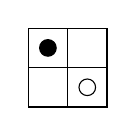
\begin{tikzpicture}[x=1cm]
			\draw (0,0)--(1,0)--(1,1)--(0,1)--cycle;
			\draw (.5,0)--(.5,.5)--(.5,1);
			\draw (0,.5)--(.5,.5)--(1,.5);
			\draw (.75,.25) circle (3pt);
			\filldraw (.25,.75) circle (3pt);
		\end{tikzpicture}
		\caption{$c_{1}$}
	\end{subfigure}%
	%c2
	\begin{subfigure}[t]{.1\textwidth}
		\centering
		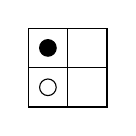
\begin{tikzpicture}[x=1cm]
			\draw (0,0)--(1,0)--(1,1)--(0,1)--cycle;
			\draw (.5,0)--(.5,.5)--(.5,1);
			\draw (0,.5)--(.5,.5)--(1,.5);
			\draw (.25,.25) circle (3pt);
			\filldraw (.25,.75) circle (3pt);
		\end{tikzpicture}
		\caption{$c_{2}$}
	\end{subfigure}%
	%c3
	\begin{subfigure}[t]{.1\textwidth}
		\centering
		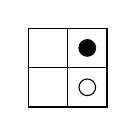
\begin{tikzpicture}[x=1cm]
			\draw (0,0)--(1,0)--(1,1)--(0,1)--cycle;
			\draw (.5,0)--(.5,.5)--(.5,1);
			\draw (0,.5)--(.5,.5)--(1,.5);
			\draw (.75,.25) circle (3pt);
			\filldraw (.75,.75) circle (3pt);
		\end{tikzpicture}
		\caption{$c_{3}$}
	\end{subfigure}%
	%c4
	\begin{subfigure}[t]{.1\textwidth}
		\centering
		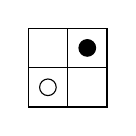
\begin{tikzpicture}[x=1cm]
			\draw (0,0)--(1,0)--(1,1)--(0,1)--cycle;
			\draw (.5,0)--(.5,.5)--(.5,1);
			\draw (0,.5)--(.5,.5)--(1,.5);
			\draw (.25,.25) circle (3pt);
			\filldraw (.75,.75) circle (3pt);
		\end{tikzpicture}
		\caption{$c_{4}$}
	\end{subfigure}%
	%c5
	\begin{subfigure}[t]{.1\textwidth}
		\centering
		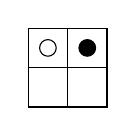
\begin{tikzpicture}[x=1cm]
			\draw (0,0)--(1,0)--(1,1)--(0,1)--cycle;
			\draw (.5,0)--(.5,.5)--(.5,1);
			\draw (0,.5)--(.5,.5)--(1,.5);
			\draw (.25,.75) circle (3pt);
			\filldraw (.75,.75) circle (3pt);
		\end{tikzpicture}
		\caption{$c_{5}$}
	\end{subfigure}%
	%c6
	\begin{subfigure}[t]{.1\textwidth}
		\centering
		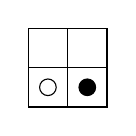
\begin{tikzpicture}[x=1cm]
			\draw (0,0)--(1,0)--(1,1)--(0,1)--cycle;
			\draw (.5,0)--(.5,.5)--(.5,1);
			\draw (0,.5)--(.5,.5)--(1,.5);
			\draw (.25,.25) circle (3pt);
			\filldraw (.75,.25) circle (3pt);
		\end{tikzpicture}
		\caption{$c_{6}$}
	\end{subfigure}
	
	%c7
	\begin{subfigure}[t]{.1\textwidth}
		\centering
		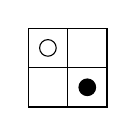
\begin{tikzpicture}[x=1cm]
			\draw (0,0)--(1,0)--(1,1)--(0,1)--cycle;
			\draw (.5,0)--(.5,.5)--(.5,1);
			\draw (0,.5)--(.5,.5)--(1,.5);
			\draw (.25,.75) circle (3pt);
			\filldraw (.75,.25) circle (3pt);
		\end{tikzpicture}
		\caption{$c_{7}$}
	\end{subfigure}%
	%c8
	\begin{subfigure}[t]{.1\textwidth}
		\centering
		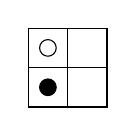
\begin{tikzpicture}[x=1cm]
			\draw (0,0)--(1,0)--(1,1)--(0,1)--cycle;
			\draw (.5,0)--(.5,.5)--(.5,1);
			\draw (0,.5)--(.5,.5)--(1,.5);
			\draw (.25,.75) circle (3pt);
			\filldraw (.25,.25) circle (3pt);
		\end{tikzpicture}
		\caption{$c_{8}$}
	\end{subfigure}%
	%c9
	\begin{subfigure}[t]{.1\textwidth}
		\centering
		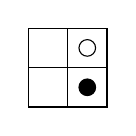
\begin{tikzpicture}[x=1cm]
			\draw (0,0)--(1,0)--(1,1)--(0,1)--cycle;
			\draw (.5,0)--(.5,.5)--(.5,1);
			\draw (0,.5)--(.5,.5)--(1,.5);
			\draw (.75,.75) circle (3pt);
			\filldraw (.75,.25) circle (3pt);
		\end{tikzpicture}
		\caption{$c_{9}$}
	\end{subfigure}%
	%c10
	\begin{subfigure}[t]{.1\textwidth}
		\centering
		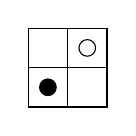
\begin{tikzpicture}[x=1cm]
			\draw (0,0)--(1,0)--(1,1)--(0,1)--cycle;
			\draw (.5,0)--(.5,.5)--(.5,1);
			\draw (0,.5)--(.5,.5)--(1,.5);
			\draw (.75,.75) circle (3pt);
			\filldraw (.25,.25) circle (3pt);
		\end{tikzpicture}
		\caption{$c_{10}$}
	\end{subfigure}%
	%c11
	\begin{subfigure}[t]{.1\textwidth}
		\centering
		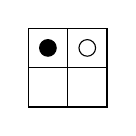
\begin{tikzpicture}[x=1cm]
			\draw (0,0)--(1,0)--(1,1)--(0,1)--cycle;
			\draw (.5,0)--(.5,.5)--(.5,1);
			\draw (0,.5)--(.5,.5)--(1,.5);
			\draw (.75,.75) circle (3pt);
			\filldraw (.25,.75) circle (3pt);
		\end{tikzpicture}
		\caption{$c_{11}$}
	\end{subfigure}%
	%c12
	\begin{subfigure}[t]{.1\textwidth}
		\centering
		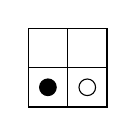
\begin{tikzpicture}[x=1cm]
			\draw (0,0)--(1,0)--(1,1)--(0,1)--cycle;
			\draw (.5,0)--(.5,.5)--(.5,1);
			\draw (0,.5)--(.5,.5)--(1,.5);
			\draw (.75,.25) circle (3pt);
			\filldraw (.25,.25) circle (3pt);
		\end{tikzpicture}
		\caption{$c_{12}$}
	\end{subfigure}
	
	%D
	\begin{subfigure}[b]{\textwidth}
		\centering
		\[D:
		\raisebox{-.5\height}
		{
			\begin{tikzpicture}[every edge/.style={draw,postaction={decorate,decoration={markings,mark=at position 0.5 with {\arrow[scale=2]{>}}}}}]
				\foreach \i/\j in {0/12,1/11,2/10,3/9,4/8,5/7,6/6,7/5,8/4,-3/3,-2/2,-1/1} {
					\setcounter{Angle}{90 + \i * 360 / 12};
					\vertex (c\j) at (\theAngle:2) [label=\theAngle:$c_{\j}$]{};
				}
				\path
					(c1) edge[bend right=40] (c3)
					(c1) edge[bend left=40] (c11)
					(c2) edge (c1)
					(c2) edge[bend right=40] (c4)
					(c4) edge (c3)
					(c4) edge (c5)
					(c6) edge[bend left=40] (c4)
					(c6) edge (c7)
					(c7) edge[bend left=40] (c5)
					(c7) edge[bend right=40] (c9)
					(c8) edge (c7)
					(c8) edge[bend right=40] (c10)
					(c10) edge (c9)
					(c10) edge (c11)
					(c12) edge[bend left=40] (c10)
					(c12) edge (c1)
				;
			\end{tikzpicture}
		}\]
	\end{subfigure}
	\caption{Modeling twelve configurations by a digraph}
\end{figure}

\begin{exers}\end{exers}

\begin{exer}
\begin{enumerate}[{(a)}]
\item Let $S = \{2,3,4,7,11,13\}$. Construct the multigraph $M$ whose vertex set is $S$ and where $ij$ is an edge for distinct elements $i$ and $j$ in $S$ whenever $i+j \in S$ and $ij$ is an edge whenever $|i-j| \in S$. In other words, $i$ and $j$ are joined by two edges if both $i+j \in S$ and $|i-j| \in S$.
\item How are the problem and solution in (a) affected if we remove the word "distinct"?
\end{enumerate}
\end{exer}

\begin{exer}
Consider the twelve configurations $c_{i}$, $1 \leq i \leq 12$, in Figure 1.38. Draw the digraph $D$, where $V(D) = \{c_{1},c_{2},\ldots,c_{12}\}$ and where $(c_{i},c_{j})$ is a directed edge of $D$ if it is possible to obtain $c_{j}$ by rotating the configuration $c_{i}$ either $\degree{90}$ or $\degree{180}$ clockwise about the midpoint of the checkerboard.
\end{exer}

\begin{exer}
Using the twelve configurations in Figure 1.38, define a transformation different from the one described in Exercise 1.30 which can be modeled by a digraph but not by a graph.
\end{exer}

\begin{exer}
Let $S$ and $A$ be two finite nonempty sets of integers. Define a digraph $D$ with $V(D) = A$, where $(x,y)$ is an arc of $D$ if $x \neq y$ and $y-x \in S$.
\begin{enumerate}[{(a)}]
\item Draw the digraph $D$ for $A = \{0,1,2,3,4\}$ and $S = \{-2,1,2,4\}$.
\item What can be said about $D$ if $A$ and $S$ consist only of odd integers?
\item How can the question in (b) be generalized?
\item If $|A| = |S| = 5$, how large can the size of $D$ be?
\end{enumerate}
\end{exer}

\begin{exer}
A digraph $D$ has vertex set $\{-3,3,6,12\}$ and $(i,j) \in E(D)$ if $i \neq j$ and $i \div j$, that is, $j$ is a multiple of $i$. Draw the digraph $D$.
\end{exer}